\documentclass[12pt]{article}
\usepackage[spanish]{babel}
\usepackage{geometry}
\geometry{a4paper, margin=1in}
\usepackage{graphicx}
\usepackage{xcolor}
\usepackage{titlesec}
\usepackage{parskip}
\usepackage{multicol}
\usepackage{cite}
\usepackage{listings}
\usepackage{color}
\usepackage{amsmath}
\usepackage{enumitem}

\lstset{
  language=Python,
  basicstyle=\ttfamily\small,
  keywordstyle=\color{blue},
  commentstyle=\color{gray},
  stringstyle=\color{red},
  breaklines=true,
  showstringspaces=false
}


\definecolor{highlight}{RGB}{255, 255, 0}

\titleformat{\section}{\normalfont\Large\bfseries}{\thesection}{1em}{}
\titleformat{\subsection}{\normalfont\large\bfseries}{\thesubsection}{1em}{}

\begin{document}

% Logos
\begin{minipage}{0.45\textwidth}
    
\includegraphics[width=0.4\textwidth]{inFiles/Figures/epnLogo.jpg}
\end{minipage}
\hfill
\begin{minipage}{0.45\textwidth}
    \raggedleft
    
\includegraphics[width=0.4\textwidth]{inFiles/Figures/FIS_logo.jpg}
\end{minipage}

\vspace{0.5cm}

% Títulos principales
\begin{center}
    \textbf{ESCUELA POLITÉCNICA NACIONAL}\\[0.2cm]
    \textbf{FACULTAD DE INGENIERÍA DE SISTEMAS}\\[0.2cm]
    \textbf{INGENIERÍA EN CIENCIAS DE LA COMPUTACIÓN}
\end{center}

\vspace{0.5cm}
\hrule
\vspace{0.5cm}

% Datos principales
\noindent\textbf{PERÍODO ACADÉMICO:} 2025-A\\[0.2cm]
\noindent\textbf{ASIGNATURA:} ICCD412 Métodos Numéricos \hfill \textbf{GRUPO:} GR2\\[0.2cm]
\noindent\textbf{TIPO DE INSTRUMENTO:} Práctica3\\[0.2cm]
\noindent\textbf{FECHA DE ENTREGA LÍMITE:} {07/05/2025}\\[0.2cm]
\noindent\textbf{ALUMNO:} {Sebastián Chicaiza}

\vspace{0.5cm}
\hrule
\vspace{1cm}


% Secciones
\section*{TEMA}

\begin{center}
    \Large\textbf{Método de la bisección}
\end{center}
\vspace{0.5cm}

\section*{OBJETIVOS}
\begin{itemize}
    \item {Conocer como aplicar el método de la bisección para sacar soluciones aproximadas a ecuaciones no lineales.}
    \item {Analizar el comportamiento y la presición del método de la bisección.}
\end{itemize}
\vspace{0.5cm}
\section*{MARCO TEÓRICO}
El método de la bisección es un proceso iterativo que consiste en evaluar una funcion \(f(x)\) en el punto medio \(p\) de un intervalo de interés \((x_1,x_2)\).
Dependiendo si su ordenada tiene el mismo signo que \(f(p)\) o no, se definirá que punto limite del intervalo tomará el valor \(p\) en la siguiente iteración. 
Este proceso se repetirá hasta que el intervalo esté dentro de un rango aceptable de error, es decir menor que una toleracia prefijada\cite{mathews2000metodos}.

Para aplicar el método de la bisección se utilizan los siguientes teoremas:

\textbf{Teorema del valor intermedio}

Si \(f \in C[a,b]\) y \(K\) es cualquier número entre \(f(a)\) y \(f(b)\), entonces existe un número \(c\) en \((a,b)\) para el cual \(f(c) = K\).

\textbf{Búsqueda de cambio de signo}

Un intervalo \([a,b]\), la función \(f(x)\) toma valores de diferente signo en los extremos.
\[f(a) \cdot f(b) < 0\]

\section*{DESARROLLO}

\subsection*{Ejercicios Aplicados}

\begin{enumerate}
    \item Un abrevadero de longitud \(L\) tiene una sección transversal en forma de semicírculo con radio \(r\). (Consulte la
    figura adjunta.) Cuando se llena con agua hasta una distancia \(h\) a partir de la parte superior, el volumen \(V\) de
    agua es
    \[V = L \left[ 0.5\pi r^{2} - r^{2}\arcsen{\left( \frac{h}{r} \right)} - h(r^{2} - h^{2})^{1/2} \right]\]
    \begin{center}
        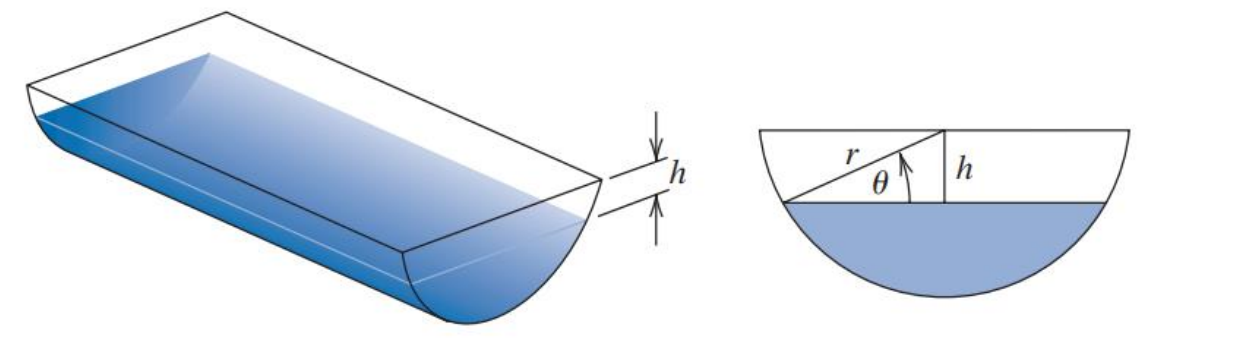
\includegraphics[width=0.9\textwidth]{inFiles/Figures/ej1Biseccion.png} 
    \end{center}

    Suponga que \(L = 10 cm\), \(r = 1 cm \) y \(V = 12.4 cm^{3}\). Encuentre la profundidad del agua en el abrevadero dentro de \(0.01 cm\).

    \item Un objeto que cae verticalmente a través del aire está sujeto a una resistencia viscosa, así como a la fuerza
    de gravedad. Suponga que un objeto con masa \(m\) cae desde una altura \(s_0\) y que la altura del objeto después
    de \(t\) segundos es
    \[s(t) = s_0 - \frac{mg}{k}t + \frac{m^{2}g}{k^{2}} \left( 1- e^{-kt/m}\right)\],
    donde \(g = 9.81 m/s^{2}\) y \(k\) representa el coeficiente de la resistencia del aire en \(\frac{Ns}{m}\). Suponga \(s_0 = 300m\),
    \(m = 0.25 kg\) y \(k = 0.1 \frac{Ns}{m}\). Encuentre, dentro de \(0.01 segundos\), el tiempo que tarda un cuarto de \(kg\) en golpear el piso. 
\end{enumerate}

\subsection*{Ejercicios Teóricos}

\begin{enumerate}       
    \item Use el teorema 2.1 para encontrar una cota para el número de iteraciones necesarias para lograr una
    aproximación con precisión de \(10^{-4}\) para la solución de \(x^{3} -x -1 = 0\) que se encuentra dentro del intervalo
    \([1, 2]\). Encuentre una aproximación para la raíz con este grado de precisión.

    \item La función definidapor \(f(x) = \sin{\pi} x\) tiene ceros en cada entero. Muestre cuando \(-1 < a< 0\) y \(2 < b< 3\),
    el método de bisección converge a

    \begin{enumerate}[label=\alph*.]
        \item \(0, si \quad a+b<2\)
        \item \(2, si \quad a+b>2\)
        \item \(1, si \quad a+b=2\)
    \end{enumerate}
\end{enumerate}     
\section*{CONCLUCIONES}
\begin{itemize}
    \item {La conversion a formato IEEE 754 de 64 bits permite representar una gran cantidad de valores con alta presición.}
    \item {El resultado del cálculo del error relativo de la conversión demuestra la presición de este formato.} 
\end{itemize}

\section*{RECOMENDACIONES}

Tener en cuenta el valor del error relativo al utilizar el formato IEEE 754 para representar números.
Especialmente cuando se trata de resultados en el campo científico, donde se requiere de gran presición.
\renewcommand{\refname}{\MakeUppercase{REFERENCIAS}}
\bibliographystyle{IEEEtran}
\bibliography{inFiles/References/references.bib}


\end{document}
